\chapter{Blockchain Notarization with OpenTimestamps}
\label{chpr:notarization}

We devoted Chapter \ref{chpr:consensus} and Chapter \ref{chpr:btc} in understanding how Bitcoin achieves distributed consensus, thus convincing ourselves that the relative blockchain is, in geek speak, \textit{immutable}. We made this effort to lay the foundations for one of the most interesting non-monetary application\footnote{Behind the hype for the blockchain in the current years as the definitive solution of all the world's problems, notarization of digital documents stands out as one of the few real applications of this technology.} of the blockchain, that is the \textit{notarization} of digital documents. According to National Notary Association\footnote{More details in the official website: \url{https://www.nationalnotary.org/knowledge-center/about-notaries/what-is-notarization}.}:

\bigskip
\noindent
\enquote{Notarization is the official fraud-deterrent process that assures the parties of a transaction that a document is authentic, and can be trusted. It is a three-part process, performed by a Notary Public, that includes of vetting, certifying and record-keeping.}

\bigskip
\noindent
Traditionally, the notarization process is achieved by certification authorities (CA), like notary public or banks, because of their reliability. It is only thanks to the relationship of trust with social organizations if this task is possible. The majority of notary services are based on ledgers attesting non-repudiable and non-alterable transactions between two counterparts.

\bigskip
\noindent
However, a central authority represents a single point of failure. Who maintains that ledger could act maliciously and easily tamper some data for his own interest. Hence the need to decentralize the source of trust and grant the reliability of that ledger even if the security of the aforementioned central authority breaks from the inside. A careful reader will have already figured out that the blockchain is the technology that perfectly fits our interest, assuring tamper-resistance and non-repudiation of data written in the chain. Among them, permissionless (public) blockchain is more preferred, because a service built on top of a permissioned (private) blockchain represents a single point of failure, as for a central authority. So, it results that the Bitcoin blockchain is the right answer\footnote{Regarding this, Italian law recognizes the validity of blockchain notarization and AGID will have to specify technical detail. \\ More info here: \url{https://www.agendadigitale.eu/documenti/blockchain-nel-ddl-semplificazioni-conseguenze-e-problemi-dellattuale-testo/}}. Unfortunately, at least for now, it cannot replace all the notary services, but it is perfect to give \textit{proof-of-existance} of a document, a procedure usually called \textit{timestamping}.

\bigskip
\section{Blockchain Timestamping}
A timestamp can be seen as a sequence of characters representing the time in which an event occurred. Hence, timestamping is an increasingly valuable complement to digital signing practices, enabling organizations to record when a digital item, such as a message, document, transaction or piece of software, was signed. In addition, the timing of a digital signature is critical in many cases, like lottery ticket issuance and some legal proceedings. Even when time is not intrinsic to the application, timestamping is helpful for record keeping and audit processes, because it proves whether the digital certificate was valid at the time it was used. More precisely:

\begin{mydef}{\bf (timestamp)}.
    A timestamp is a proof that some data d existed prior to a certain time t.
\end{mydef}

\bigskip
\noindent
To create such proof, $d$ has to cause an event that could not have been
generated without the existence of $d$. Such event must be attested to time $t$ and
can be publicly observed. So a proof consists in the data $d$, the set of operations binding $d$ to the time $t$, and the time attestation. However, we have to deal with the fact that digital documents can be easily falsified without leaving any trail of tamper evidence. Hence, a \enquote{good} timestamp proof must become invalid even if a single bit of the input string is modified. Once again cryptography comes in help and the creation procedure of a timestamp proof does not require to publish $d$ on the blockchain, but only a \textit{commitment} to it, that is something caused by the input $d$ or, in other words, something that follow such input in time. Let us be a little bit more precise:
\begin{mydef}{\bf (commitment operation)}.
    A function $C: X \rightarrow Y$ is a commitment operation if given $x_{1} \in X$ it is not feasible to compute $x_{2} \in X$ s.t. $x_{1} \neq x_{2}, C(x_{1}) = C(x_{2})$.
\end{mydef}

\bigskip
\noindent
Recalling Definition \ref{def:hash-prop}, requiring a function to be a \textit{commitment} operation is the same to require that function to fulfill \textit{second-preimage resistance}, a property already seen in Paragraph \ref{sub:hash} for hash functions. We will now provide some simple examples of commitment operations in order to understand better, the \enquote{\textit{append}} and \enquote{\textit{prepend}} operations.
\begin{myexample}{\bf (\enquote{append})}.
    \textquotedblleft hello\textquotedblright $\xrightarrow{\text{append(\textquotedblleft world\textquotedblright)}}$ \textquotedblleft helloworld\textquotedblright.
\end{myexample}
\begin{myexample}{\bf (\enquote{prepend})}.
    \textquotedblleft world\textquotedblright $\xrightarrow{\text{prepend(\textquotedblleft hello\textquotedblright)}}$ \textquotedblleft helloworld\textquotedblright.
\end{myexample}

\bigskip
\noindent
It is clear that these commitment operations bind inputs to outputs, thus making impossible to tamper the inputs without any evidence in the outputs. However, any user of a timestamp service would have its privacy respected, thus not revealing the content of the data $d$, a property that neither \enquote{\textit{append}} nor \enquote{\textit{prepend}} are able to provide. In addition, the outputs of these specific operations are always bigger in size than the inputs, not a good feature if we want to record such commitments in the blockchain, having blocks strict size limits.

\bigskip
\noindent
To address these issues, we need a tailored commitment operation that fits our case, that is the \textit{hash function}. As we already saw in Paragraph \ref{sub:hash}, hash functions achieve specific properties:
\begin{itemize}
    \item The same input data $d$ will always yield the same hash value.
    \item The hash value is always of a fixed length\footnote{Accordingly to the Bitcoin protocol, we will use SHA256, resulting in a 256-bits output length.}, no matter what size of the input data $d$.
    \item Any change in the input data $d$, even a single bit, will have a totally different hash value and therefore can be detected.
    \item It is impossible to recover the original data $d$ from the hash value, so it hides the input.
\end{itemize}

\bigskip
\noindent
Now that we have seen all the properties a good commitment operation must achieve, what is left is to learn how blockchain timestamp effectively works.

\bigskip
\noindent
Hash functions, like SHA256, are implemented as open algorithms, so any client can \enquote{hash} the document he wants to timestamp from any computer and using any programming languages, without the need to trust any third party for this task.

\bigskip
\noindent
Once the hash value is computed, it can be associated to a particular Bitcoin transaction, called \textit{null data transaction}. This specific type of transaction makes use of OP\_RETURN, an opcode script introduced in the Bitcoin Core 0.9.0 release. It allows to add arbitrary data to a provably unspendable pubkey script that full nodes do not have to store in their UTXO dataset. This feature is good at preventing the UTXO dataset to bloat. From Bitcoin Core 0.11.0, \textit{null data transactions} are relayed and mined with up to 80 bytes\footnote{From version 0.9.x to 0.11.x of the Bitcoin Core, the size for pushing arbitrary data in the null data transaction was 40 bytes.} in a single data push with the limitation of one null data output paying exactly 0 satoshis\footnote{Amounts in Bitcoin are expressed in \textit{satoshi}, currently the smallest unit of the bitcoin currency recorded on the blockchain, i.e. $10^{-8}$ bitcoin.}: 
\begin{verbatim}
Pubkey Script: OP_RETURN <0 to 80 bytes of data>
\end{verbatim}
This \textit{null data script} cannot be spent, so there is not an associated \textit{unlocking script}. Then, the aforementioned transaction is broadcast to the network, waiting for a miner to add it in the transaction set of a mined block. We already saw that a block header contains a specific field called \textit{merkleroot} when we talked about mining in Paragraph \ref{par:pow}, substantially the root of a binary tree that summarize all the transactions in that block or, in other words, a \textit{commitment} to them. We will use this tree structure, called \textit{merkle tree}\textup{\footnote{The name \textit{merkle tree} comes from Ralph Merkle, who patented it in 1979.}}, in the next chapters, thus we will give here a brief explanation:

\begin{mydef}{\bf (merkle tree)}.
    \label{def:merkle}
    In cryptography and computer science, a binary hash tree or merkle tree is a tree in which every leaf node is labelled with the hash of a data block, and every non-leaf node is labelled with the cryptographic hash of the labels of its two child nodes.
\end{mydef}

\bigskip
\noindent
The simple way to fix in mind such a structure is by a figure. Antonopoulos in his book \enquote{Mastering Bitcoin} \cite{Antonopoulos:2017:MBP:3164842} did it for us.

\begin{figure}[ht]
    \centering
	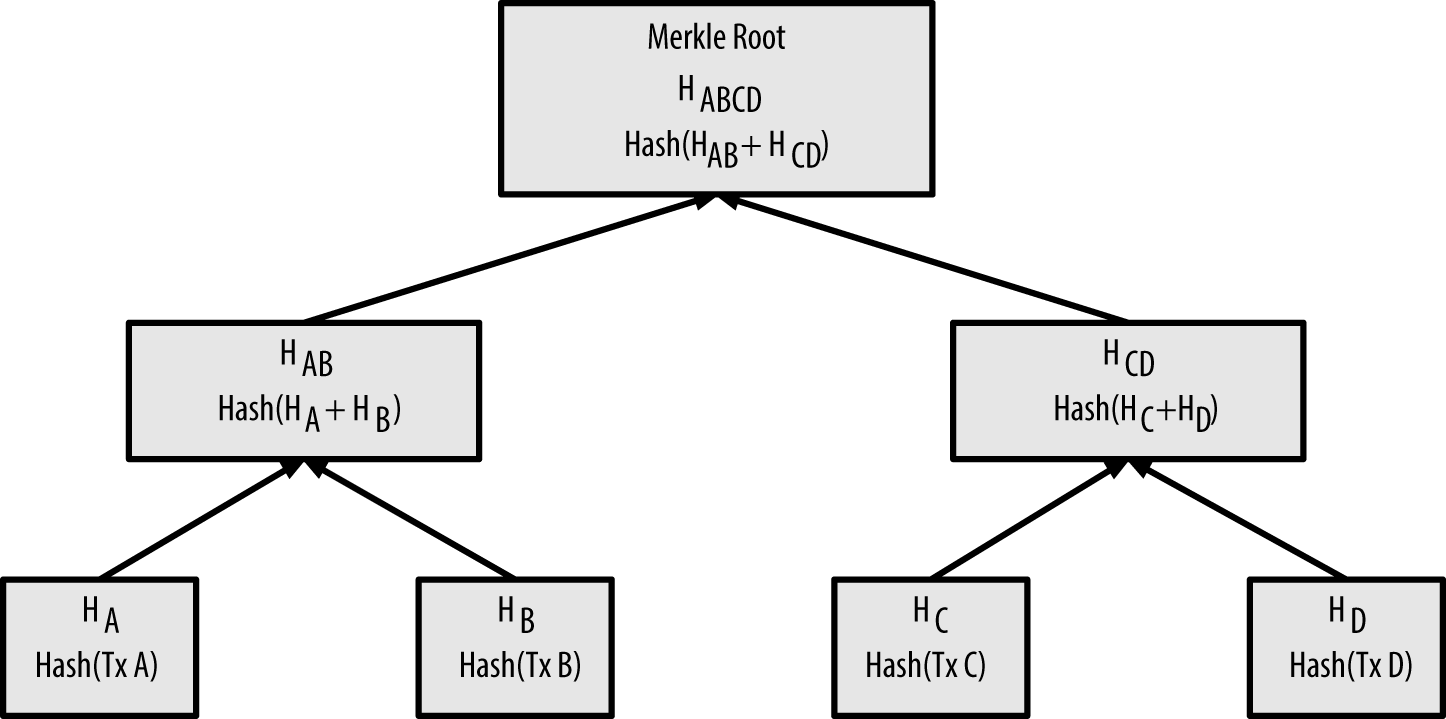
\includegraphics[width=0.9\linewidth]{Images/merkle-tree.png}
	\caption{An example of a merkle tree of transactions}
	\label{fig:merkle}
	\source{\url{https://github.com/bitcoinbook/bitcoinbook/blob/develop/images/mbc2_0902.png}}
\end{figure}

\bigskip
\noindent
A careful reader will already have understood that, in our case, data in Definition \ref{def:merkle} are transactions and the hash function used  is SHA256. Hence, for the properties of hash functions, the \textit{merkleroot}, so the block header commits to all the transactions in a block, also to the specific one that in turn commits to the data to timestamp. 

\bigskip
\noindent
Finally, thanks to what we have learned in the previous chapters, we can think of the Bitcoin network as a decentralized, trustless, permissionless notary. Its attestations are stored in the blockchain, a widely published and immutable timestamps chain\footnote{We recall that a block header also contains a \textit{time} field, a Unix epoch time when the miner started hashing the header (according to the miner). Its value must be strictly greater than the median time of the previous 11 blocks. Full nodes will reject blocks with headers more than two hours in the future according to their clock. This definition is taken from \url{https://bitcoin.org/en/developer-reference\#block-headers}.}. It is this immutability to provide timestamping, proving the data file existence at that moment in time in that specific status. Manca immagine timestamp.

\bigskip
\noindent
Summing up, blockchain timestamping provides a public proof of existence of a digital document, that cannot be faked or removed and without the need of a central trusted authority. In addition, it can be used along with timestamping prescription. However, this procedure has some downsides, being not efficient (it needs a transaction per timestamp) and lacking a proper standardization. But, in 2012 Peter Todd started working on an open-source project\footnote{The earliest Git commits date back to June 2012, as you can see here: \url{https://github.com/opentimestamps/opentimestamps-server/commit/6e2519d0bb8af2c6ec006e7849d626b20af99a77}.}, called \textit{OpenTimestamps} \cite{OTSWeb}, that aims to provide a standard format for blockchain timestamping, and efficiently resolves these downsides.

\bigskip
\section{OpenTimestamps}
\label{sec:ots}
\textit{OpenTimestamps} defines a set of rules for conveniently creating provable timestamps and later independently verifying them. Currently this protocol fully supports Bitcoin blockchain timestamping, however it is flexible enough to support timestamping on other blockchains like Ethereum and Litecoin. Obviously such a proof is reliable as the chain committing to it, hence without a doubt the Bitcoin one is nowadays the best choice.

\bigskip
\noindent
A timestamp proof made with \textit{OpenTimestamps} consists in a list of commitment operations applied in sequence to the document, ending with one or more time attestations. Such a list of operations is actually a tree of operations, with the document as the root, the commitment operations as the edges and time attestations as the leaves. Anyone can easily verify the proof just replaying the operations and checking that the final result is a message that you already know existed at a certain time. Since commitment operations grant that different inputs will always result in different outputs, we are sure that there is no way to change the original document without invalidating the proof.

\bigskip
\subsection{Solving Scalability Problem}
As we mentioned before, \textit{OpenTimestamps} proposes a solution to the scalability problem, allowing to efficiently aggregate possibly up to an infinite number of documents to timestamp in a single transaction, a feature non supported by most of the existing timestamping services. The trick is to compose those documents in a \textit{merkle tree} and to push its \textit{merkleroot} into a transaction, as the classic blockchain timestamping solutions did for a single hash value. Hence, each per-document proof is just the path up to the first merkle tree composed by documents' hashes, then up to the merkle tree of transactions, reaching the merkleroot in the block header which alone is a commitment to all the documents.

\begin{figure}[ht]
    \centering
	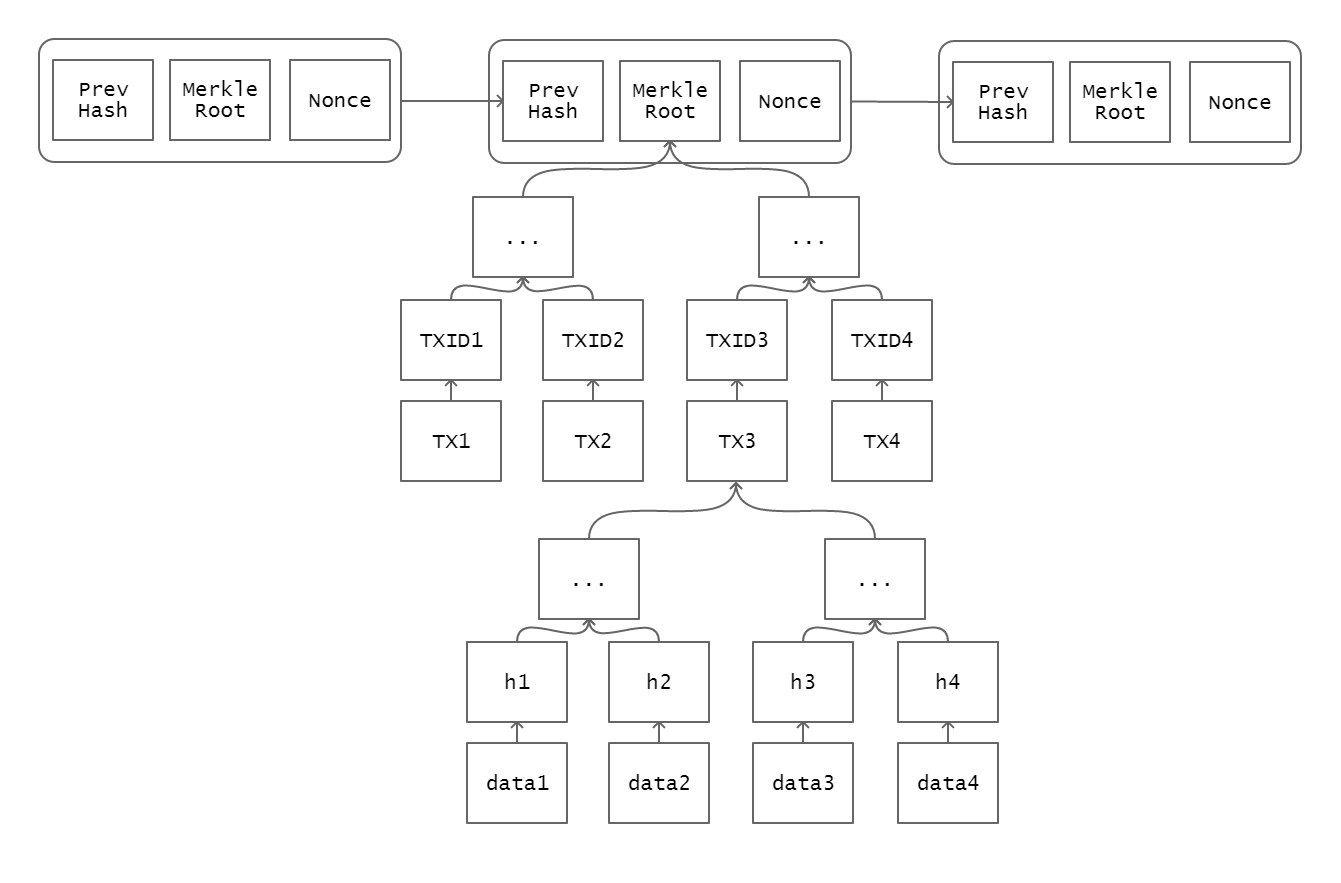
\includegraphics[width=0.9\linewidth]{Images/bitcoin-chain-calendar.png}
	\caption{Scalability solution with \textit{OpenTimestamps}.}
	\label{fig:scalability}
	\source{\cite{Comandini:Thesis:2018}}
\end{figure}

\bigskip
\noindent
In addition to this, \textit{OpenTimestamps} comes with a system of \textit{aggregation servers}\textup{\footnote{Examples of public \textit{aggregation servers} are: \url{a.pool.opentimestamps.org} and \url{b.pool.opentimestamps.org}.}}, publicly available \enquote{meeting points}, where anyone can submit a digest to be timestamped, as Peter Todd said in \cite{OTSannouncment}. As its name suggests, an aggregation server collects documents' hash values in a pending list of digests and periodically \textit{aggregates} these digests into a single merkle tree. Notice that the aggregation server learns nothing about the original documents, it only collects \enquote{meaningless} digests\footnote{In the sense that there is no way to retrieve the original document from its hash value.}. In addition each file is protected by a nonce, thus files are not directly connected in any way. Then, the root of that tree is timestamped with Bitcoin. But there is a little price to pay, aggregation servers are obviously centralized and represent single points of failure because they could go offline, stopping the service. However this represents just a little inconvenience, aggregation servers remain \textit{trustless} in the sense that they cannot tamper a proof, because it is Bitcoin and not theirselves to provide the validity of a timestamp.

\newpage
\noindent
The real downside is that aggregation servers are extremely efficient but not convenient. To obtain a proof, even if for more documents at once, you have to wait for the transaction committing to the document to confirm, that is 10 minutes on average if it is included in the next block. That is too much time in many cases, for example in a timestamped e-mails exchange.

\bigskip
\noindent
But there is a compromise to address this problem which allows any user to receive such proof almost instantly: public \textit{calendar servers}. A \textit{calendar server} grants remote access to a \textit{calendar}, a collection of timestamps. Calendar servers and aggregation servers work in conjunction: rather than timestamping the tip\footnote{We use the word \textit{tip} as a synonym of \textit{root}, hence whenever the word \textit{merkletip} will appear, it indicates the root of that merkle tree.} of the merkle tree of digests directly with Bitcoin, aggregation servers aggregate pending digests in a one second interval into a merkle tree and submit the tip of that tree to a public calendar server. The latter makes the promise that every submitted merkletip will be timestamped by the Bitcoin blockchain in a reasonable amount of time, and keeps indefinitely all completed timestamps, publicly available in every moment. Hence, the proof is generated in about one second. Obviously, the inconvenience here is that public calendar servers are, as aggregation servers before, a central point of failure. In fact, a proof made with the aid of a calendar server is called \textit{incomplete}. However, once the Bitcoin blockchain has definitely completed the timestamp, such incomplete proof can be \textit{upgraded}, adding the path up to the block header merkletip, but we will go into details later in this chapter. Algorithm \ref{alg:calendar-working}, a slight modification of the one proposed by L. Comandini in his master thesis work \cite{Comandini:Thesis:2018}, perfectly describes how calendar and aggregation servers cooperate.

\begin{algorithm}
	\caption{Cooperation between aggregation and calendar servers}
	\label{alg:calendar-working}
	\begin{algorithmic}[1]
		\State clients send data to timestamp to the aggregator\footnotemark \Comment{timestamp requests}
		\State aggregator composes a merkle tree of digests each second\Comment{aggregation}
		\State aggregator sends to calendar the merkletip to timestamp
		\State calendar promise he will timestamp the tip\Comment{pending attestation}
		\State aggregator sends back to clients incomplete proof until the tip
		\State calendar aggregates pending tips in a merkle tree\Comment{aggregation}
		\State calendar sends a transaction including a merkletip\Comment{timestamp}
		\State the transaction gets confirmed \Comment{attestation complete}
		\State clients ask to the calendar to upgrade the timestamp\Comment{upgrade}
		\State calendar sends back clients the complete proofs
		\State clients verify their proofs\Comment{verification}
	\end{algorithmic}	
\end{algorithm}
\footnotetext{The term \textit{aggregator} stands for aggregation server.}

\newpage
\noindent
One last question needs to be answered: who really pays for the transactions in which digests to be timestamped are pushed in? A calendar spends bitcoins from its own wallet, making \textit{replace-by-fee}\textup{\footnote{In Bitcoin, unconfirmed transactions (yet in the mempool) can be modified and re-issued with higher fees for the miners. This leads to a higher probability for that transaction to be mined.}} transactions in order to spend a fixed amount each day. Briefly, the calendar makes a transaction with the lowest possible fees, recursively increasing that amount by a parameter $a$, fixed by who effectively runs the calendar server, until the transaction enters in a block. This result in a fixed amount of $144 \cdot a$ fees spent by the calendar each day, counting a block every 10 minutes on average. It could happen that some timestamps takes too long to be completed, a price that a user willingly pay for a service that allows completely free timestamping.

\bigskip
\noindent
What remains to be done is to learn how to practically timestamp a document with \textit{OpenTimestamps}, which provides users multiple and easy way to create and independently verify timestamps, directly from the official web page \cite{OTSWeb} or with command-line tools. We will now provide a step-by-step guide to use both the web page and the Python version of the client\footnote{\textit{OpenTimestamps} client comes in many programming languages: Python, Java, JavaScript and Rust. Here we present only the Python version because the main reference library of the project is written in Python.}.

\bigskip
\section{OpenTimestamps Python client}
\textit{OpenTimestamps} client is a command-line\footnote{Here we are supposing a Unix-based operative system.} tool to create and validate timestamp proofs, with the Bitcoin blockchain as a notary. This section is aimed to be a step-by-step tutorial to fully manage the Python release of this client\footnote{The presented guide refers to the Git repository \textit{opentimestamps-client} from the \textit{OpenTimestamps} source code \cite{OpenTimestampsGithub}.}.

\bigskip
\noindent
Before installing the \textit{OpenTimestamps} client, we must specify that while you can \textit{create} timestamps without a local Bitcoin Core node, to \textit{verify} proofs you need one\footnote{For the details about running a Bitcoin node on your local machine, see Appendix \ref{app:A}.} (a pruned node is fine too). Standing the above consideration, the increased difficulty in using a command-line tool rather than a web interface is rewarded by a complete decentralization, you do not have to rely on any third part.

\begin{itemize}
\item Install client (Python3 required):\bigskip
\begin{lstlisting}
 $ pip3 install opentimestamps-client
\end{lstlisting}
\item Install the necessary dependencies:\bigskip
\begin{lstlisting}
 $ sudo apt-get install python3 python3-dev python3-pip python3-setuptools python3-wheel
\end{lstlisting}
\item Pick a file or create a new one to timestamp:\bigskip
\begin{lstlisting}
 $ cat > filename.txt
 bla bla bla ... (write what you want)
 (type CTRL+D to close the file and return to command prompt)
\end{lstlisting}
\item Timestamp your file:\bigskip
\begin{lstlisting}[breakatwhitespace=true]
 $ ots stamp filename.txt 
 Submitting to remote calendar https://a.pool.opentimestamps.org
 Submitting to remote calendar https://b.pool.opentimestamps.org
 Submitting to remote calendar https://a.pool.eternitywall.com
 Submitting to remote calendar  https://ots.btc.catallaxy.com
\end{lstlisting}
Nice! Your timestamp request is submitted to the main public calendar servers.

\bigskip
\noindent
At this time the client must have automatically downloaded in your current directory a file
with a .ots extension, named \colorbox{light-gray}{filename.txt.ots} that is the proof of your timestamp.
\item Verify the proof (local Bitcoin Core node needed):\bigskip
\begin{lstlisting}
 $ ots verify filename.txt.ots 
 Assuming target filename is 'filename.txt'
 Calendar https://bob.btc.calendar.opentimestamps.org: Pending confirmation in Bitcoin blockchain
 Calendar https://alice.btc.calendar.opentimestamps.org: Pending confirmation in Bitcoin blockchain
 Calendar https://btc.calendar.catallaxy.com: Pending confirmation in Bitcoin blockchain
 Calendar https://finney.calendar.eternitywall.com: Pending confirmation in Bitcoin blockchain
\end{lstlisting}
Notice that you can't verify immediately the aforementioned proof. In fact, the lines saying \enquote{pending confirmation} specify that the proof is \textit{incomplete}, so a verifier has to ask the remote calendars for the rest of the proof. It takes a few hours for the timestamp to get confirmed by the Bitcoin blockchain (generally 6 confirmations). You can check for the current status of your proof file with the \colorbox{light-gray}{info} command.
\item Get detailed proof information:\bigskip
\begin{lstlisting}[breakatwhitespace=true]
 $ ots info filename.txt.ots 
 File sha256 hash: 13a1f687ddb7c1a0b12adeb708a2b464c9 cfc24d5c9def4fa775cca81162feed
 Timestamp:
 append 5669aa818cc1c5bf8129d469f884fe79
 sha256
  -> append 0f2a11ae083c66674d9d0d3da049079e
     sha256
     prepend f6836f41e86344eb7e4da03fe57c3e998d13594b2a27b4 ccb86cef8ac19cf69e
     sha256
     prepend 5c502267
     append 2c767f767b02b45c
     verify PendingAttestation ('https://bob.btc.calendar.opentimestamps.org')
  -> append 675406ae56e9e40809ac587ee009067c
     sha256
     append 7690b939b5a663ea311992aadf2f182424cea544bbfb2a 837ae366ba5cc1ecf4
     sha256
     prepend 5c502266
     append 1269e2007cc47092
     verify PendingAttestation ('https://alice.btc.calendar.opentimestamps.org')
  -> append 9b10d7ec7f0af842407d2d7cbebac9ad
     sha256
     prepend 5c502267
     append da1d41ee8803dff5
     verify PendingAttestation ('https://btc.calendar.catallaxy.com')
  -> append f923446e73e3a503121a56006723a6c1
     sha256
     append c35e379ef7097a65fdbfb2a594a93c75
     sha256
     prepend 5c502266
     append c47a3b08bfc2315e
     verify PendingAttestation ('https://finney.calendar.eternitywall.com')
\end{lstlisting}
Incomplete timestamps can be upgraded using the \colorbox{light-gray}{upgrade} command which adds the path to the relative block header merkleroot to the proof. Upgrading a proof isn't always available: there must be at least one completed attestation\footnote{That is, at least one of the four public calendars in question must have received an attestation from the Bitcoin blockchain.}.
\item Upgrade the proof: \bigskip
\begin{lstlisting}[breakatwhitespace=true]
 $ ots upgrade filename.txt.ots 
 Got 1 attestation(s) from https://bob.btc.calendar.opentimestamps.org
 Got 1 attestation(s) from https://alice.btc.calendar.opentimestamps.org
 Got 1 attestation(s) from https://btc.calendar.catallaxy.com
 Got 1 attestation(s) from https://finney.calendar.eternitywall.com
 Success! Timestamp complete
\end{lstlisting}
In this case the timestamp is fully confirmed by the Bitcoin blockchain, so upgrading the proof succeeded.

\bigskip
\noindent
Now that we know for sure that timestamping succeeded, you only left to use the \colorbox{light-gray}{verify} command another time to check which block attested your timestamp (add the flag \colorbox{light-gray}{-v} to be more verbose).\bigskip
\begin{lstlisting}[breakatwhitespace=true]
 $ ots -v verify filename.txt.ots
 Assuming target filename is 'filename.txt'
 Hashing file, algorithm sha256
 Got digest 13a1f687ddb7c1a0b12adeb708a2b464c9cfc24d5c9def 4fa775cca81162feed
 Attestation block hash: 00000000000000000013e603482 1d3d85e8a8ff0217482e4b2ab602ec7ab6ce7
 Success! Bitcoin block 560604 attests existence as of 2019-01-29 CET
\end{lstlisting}
\end{itemize}

\bigskip
\section{OpenTimestamps web interface}
Rather than the more complicated client, the easiest way to perform a timestamp with \textit{OpenTimestamps} is using the web interface on the official website \cite{OTSWeb}. It obviously allows the same actions as the client does, just interacting with the \enquote{Stamp \& Verify} box. Simply, drop a file in the box to \textit{stamp} it and the service will automatically download its proof, named as the file is with a \colorbox{light-gray}{.ots} extension. The hash of the document will be calculated inside your browser, thus not requiring the user to distribute his original document to any third party, preserving privacy.

\bigskip
\begin{figure}[htbp]
    \centering
	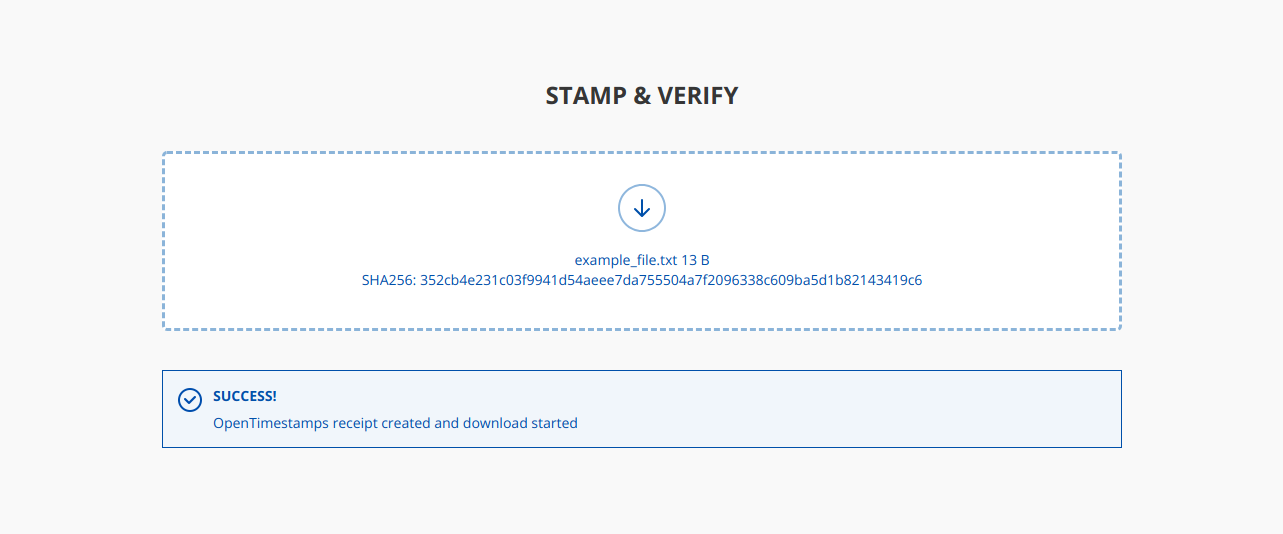
\includegraphics[width=1\linewidth]{Images/stamping.png}
	\caption{Stamping}
	\label{fig:ots-stamping}
\end{figure}

\newpage
\noindent
Alternatively, you can drop a \colorbox{light-gray}{.ots} file to \textit{verify}. Here the underlying code will detect if the file is yet in the \textit{incomplete} state and performs an \textit{upgrade}, automatically downloading the upgraded proof file. Otherwise, if the timestamp is already completed, it verifies such proof. Notice that the original document is required to start the verification process.

\bigskip
\begin{figure}[htbp]
    \centering
	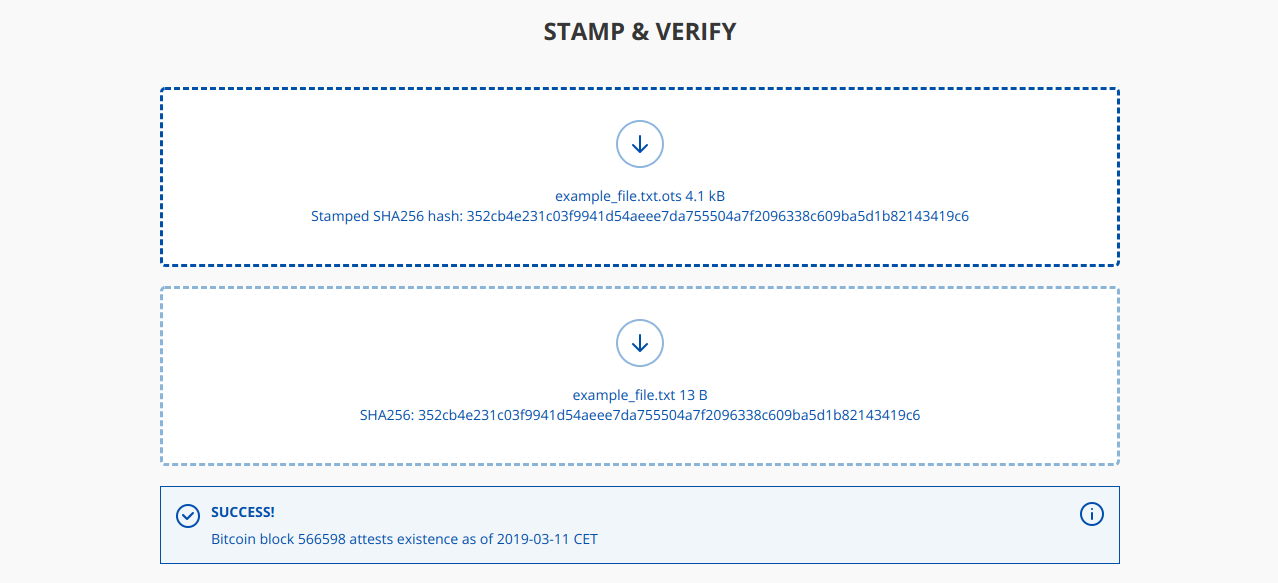
\includegraphics[width=1\linewidth]{Images/verify.png}
	\caption{Verifying}
	\label{fig:ots-verifying}
\end{figure}

\bigskip
\noindent
However, the web interface comes with a downside. Browsers applications like this one have some security restrictions, inhibiting a direct access to the local Bitcoin configuration file\footnote{We refer to Appendix \ref{app:A} for more details.}, thus preventing a user to make RPC calls to his own local Bitcoin node in order to verify a timestamp proof. Hence a user must trust the public block explorers that \textit{OpenTimestamps} uses to verify such proofs. Summing up, verification is not fully decentralized. Finally, clicking the \textit{info} button in the low right corner will open a new web page that parse the proof in a nice representation (like the \colorbox{light-gray}{info} command does for the client version, but with some added graphics).





